\documentclass{standalone}
\usepackage{tikz}
\usetikzlibrary{intersections,shapes.arrows}

\newcommand\Dist[1]{\phantom{\rule{#1}{4pt}}}

\begin{document}

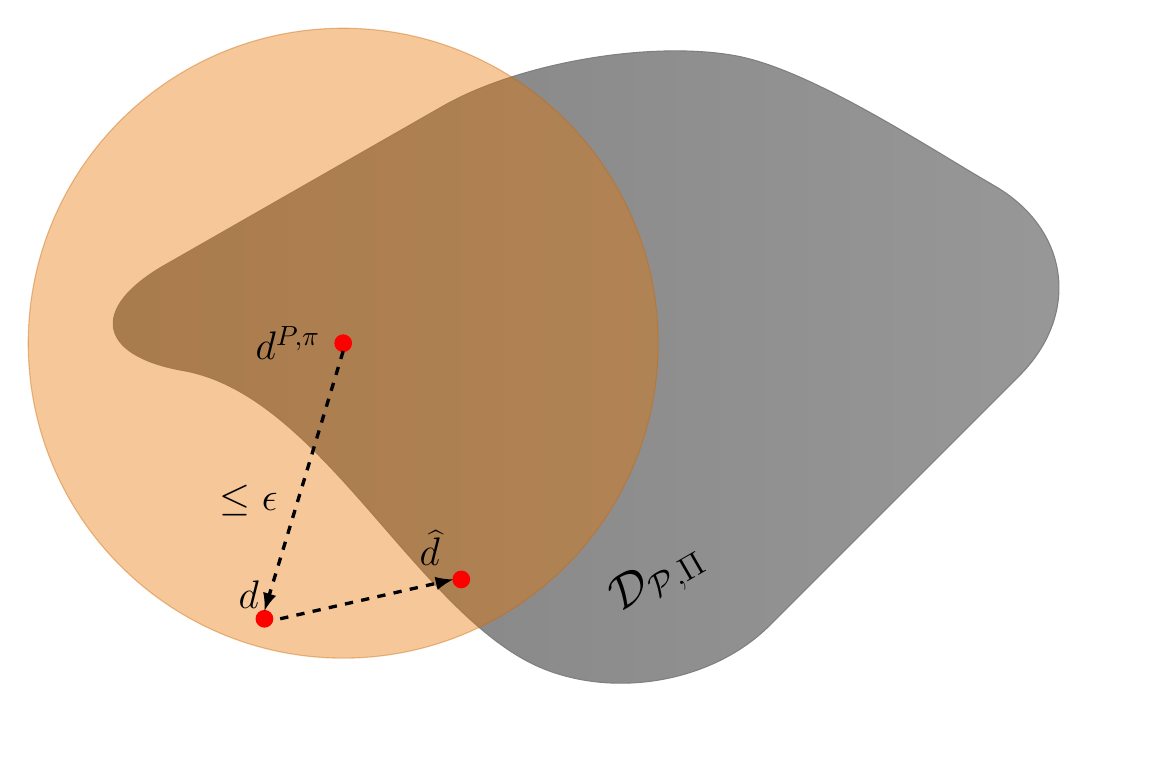
\begin{tikzpicture}
% we draw the surface
\draw[rounded corners=2cm, left color=black!50,right color=gray!80, color=gray] 
  (0,0) to[out=-10,in=150] (8,-5) -- (14,1) to[out=150,in=-10]
  (7,4) -- cycle;
  
% we add some labels
\node[rotate=30] at (8, -3) {\LARGE $\mathcal{D}_{\mathcal{P} , \Pi}$};

% trust region
\draw[color = orange!80!black, fill=orange!90!black, opacity=0.4] (4,0) circle (4cm);

%  we place the label q
\node (p) [font=\sffamily] at (3.3,0) {\Large $d^{P,\pi}$};

 % q
\draw[fill, color=red] (4,0) circle (3pt);

%  we place the label q
\node (q) [font=\sffamily] at (2.8,-3.2) {\Large $d$};

 % q
\draw[fill, color=red] (3,-3.5) circle (3pt);

\draw[name path=phatq, dashed, very thick, -latex ] (3.2,-3.5) --(5.4,-3);

\draw[name path=phatq, dashed, very thick,  -latex ](4,-0.1) -- (3,-3.4);
%  we place the label q
\node (q) [font=\sffamily] at (2.8,-2) {\Large $\leq \epsilon$};

%  we place the label q
\node (q) [font=\sffamily] at (5.1,-2.6) {\Large $\widehat{d}$};

 % q
\draw[fill, color=red] (5.5,-3) circle (3pt);

\end{tikzpicture}
\end{document}